\chapter[Solar System]{Discovering and Characterizing Small Bodies in
  the Solar System}
\def\chpname{solarsystem}\label{chp:\chpname}

Chapter editors:
\credit{rhiannonlynne},
\credit{davidtrilling}.

% ====================================================================

\section{Introduction}
\label{sec:\chpname:intro}

LSST has tremendous potential as a discovery and characterization tool
for small bodies in the Solar System. With LSST, we have the
opportunity to increase our sample sizes of Potentially Hazardous
Asteroids (PHAs), Near Earth Objects (NEOs), Main Belt Asteroids
(MBAs), Jupiter Trojans, Centaurs, TransNeptunian Objects (TNOs),
Scattered Disk Objects (SDOs), comets and other small body populations
such as Earth mini-moons, irregular satellites, and other planetary
Trojan populations, by at least an order of
magnitude, often two orders of magnitude or more. In addition to
hundreds of astrometric measurements for most objects, LSST will also
provide precisely calibrated multiband photometry. With this
information, we can also characterize these populations -- deriving
colors, light curves, rotation periods, spin states, and even shape
models where possible.

The motivation behind studying these small body populations is
fundamentally to understand planet formation and evolution. The
orbital parameters of these populations record traces of the orbital
evolution of the giant planets. The migration of Jupiter, Saturn and
Neptune in particular have left marks on the orbital distribution of
MBAs, Jupiter Trojans, TNOs and SDOs. Rapid migration of
Jupiter and Saturn may have emplaced a large number of planetesimals
in the Scattered Disk; later slow migration of Neptune will affect the
number of TNOs in resonance and the details of their orbital parameters
within the resonance. Adding color information provides further
insights; colors roughly track composition, indicating formation
location and temperature or space weathering history. For example, the color
gradient of main belt asteroids, combined with their orbital
distribution, suggests that perhaps Jupiter migrated inwards,
mixing planetesimals from the outer Solar System into the outer parts
of the main belt, before eventually migrating outwards. Studying the
size distribution of each of the small body populations themselves
provides more constraints on planetesimal formation; this is
complicated by the effects of dynamical stirring from the giant
planets, which can increase the rate of erosion vs. growth during
collisions, and by the existence of the remnants of collisions such as
collisional families in the main belt. The presence of binaries and range
of spin states and shapes provides further constraints on the history
of each population. The location
of the planets before migration, the amount of migration, and the size
distribution of the small bodies themselves (after detangling the
dynamical evolution) all tell a deeper story about how the planets in
the Solar System formed, and how our formation history fits into the
range of observed extrasolar planetary systems.

These Solar System populations are unique when compared to other
objects which will be investigated by LSST, due to the simple fact
that they move across the sky. Metrics to evaluate
LSST's performance for moving objects need to be based on `per object'
measurements, rather than at a series of points on the sky or per
field pointing. For all metrics discussed in this chapter, the orbit
of each object is integrated over the time of the simulated opsim
survey and the times when each object is visible are recorded; these
series of observations per object are then the basis for metric
evaluations.

% Introduce, with a very broad brush, this chapter's science projects,
% and why it makes sense for them to be considered together.

% ====================================================================

\section{Discovering and linking Solar System Objects}
\def\secname{\chpname:discovery}\label{sec:\secname}

Discovering, rather than simply detecting, small objects throughout
the Solar System requires unambiguously linking a series of detections
together into an orbit. The orbit provides the information necessary
to scientifically characterize the object itself and to understand the
population as a whole. Without orbits, the detections of Solar System
Objects (SSOs) by LSST will be of limited use; objects discovered with
other facilities could be followed up by LSST, but almost the entire
science benefit to planetary astronomy would be lost. Linking and
orbit determination for Solar System objects is similar to source
association for non-moving objects; it provides the means to identify
multiple detections as coming from a single object.

Therefore, the first concern regarding the Solar System is related
to the question ``Can we accurately link individual detections of moving objects into
orbits?''.  This requirement poses varying levels of difficulty as we
move from Near Earth Objects (NEOs) through the Main Belt Asteroids
(MBAs) and to TransNeptunian Objects (TNOs) and Scattered Disk Objects
(SDOs), as well as for comets and for other unusual but very
interesting populations such as Earth minimoons. Due to their small
heliocentric and geocentric distances, NEOs appear move with
relatively high velocities and are distributed over a large fraction
of the sky, far from the ecliptic plane. MBAs are densely distributed,
primarily within about 30 degrees of the ecliptic. TNOs and SDOs move
slowly, however short time intervals between repeat visits in each night may make these difficult
to link. Comets and Earth mini-moons may require more complicated
orbit fitting to allow for non-gravitational or geocentric
orbits. It also implies that we do not create false objects by
incorrectly linking detections and/or noise.

Much of the answer to this question comes down to the performance of
various pieces of LSST Data Management software. In particular,
important questions are the
rate of false positive detections resulting from difference imaging, the compute
limitations of the Moving Object Processing System (MOPS) to extend to high
apparent velocities, and the capability to unambiguously determine if
a linkage is `real' or not via orbit determination (done as part of
MOPS). Thus this question ranges beyond the limits of the OpSim simulated
surveys, but bears on the observing strategy requirements for
discovering Solar System Objects. An in-depth study of the performance
of difference imaging and MOPS is currently ongoing. However, we can
make a range of assumptions on how MOPS will perform and evaluate how
many and which objects can be linked under observational cadence, given those assumptions.


% --------------------------------------------------------------------

\subsection{Target measurements and discoveries}
\label{sec:\secname:targets}

The criteria for `discovery' with MOPS depends on the number
of observations of an object acquired per night, within some time
window (creating `tracklets'), repeated over a number of nights within window of some
days (creating `tracks'), linked into an orbit with a threshold on
astrometric residuals. The current assumptions are that we can link
detections into orbits with 2 detections per night within 90 minutes,
repeated for 3 nights within 15 days. The additional assumptions are
that with these 6 observations, we will be able to create low-accuracy orbits that will suffice to link
additional observations obtained at later (or earlier, in the LSST
archive) times, and that that the orbit fitting will enable rejection
of mislinkages.

We can also set other requirements for discovery. Requiring 4
detections within 90 minutes is a fairly common discovery criteria for
NEO surveys, as it reduces the number of mislinked tracklets to almost
zero. We could also require 4 nights of pairs, in order to improve the
initial orbit fitting and mislinkage rejection.

With these discovery criteria, we can then evaluate the completeness
of an LSST simulated survey, for a given population. We can look at
this as a function of H magnitude and as a function of orbital
parameters.

For PHAs and NEOs there are special considerations in terms of
completion that arise from planetary defense concerns. For most other
populations, the general desire is simply to have a high level of
completeness, with no gaps in completeness that depend strongly on
orbital parameters. In particular, the desire is to be able to
calibrate any selection effects in discovery so that the survey completeness can
be used to debias the underlying population models.

Discovery opportunity, and thus the completeness of the underlying
population, is very sensitive to the time interval between
observations. For most solar system objects, with a 90 minute window
within a night, gathering two or more repeat observations within a night requires
that the field pointing is revisited two or more times. Gathering
observations over multiple nights for a wide variety of Solar System
objects (moving at a wide variety of apparent velocities) generally requires covering a large
neighboring area of sky; thus the internight revisit rate for large contiguous
blocks of sky is important. An optimal discovery strategy for moving
objects could be ensuring a minimum (default: two) number of revisits
within a night within a short time window (default: 90 minutes), and
covering large contiguous amounts of sky several (default: 3) times within a
longer time window (default: 15 days).

% --------------------------------------------------------------------

\subsection{Metrics}
\label{sec:\secname:metrics}

The {\tt Discovery Metric} can be used to identify sets of detections
of a particular object that meet the defined criteria for discovery: X
detections within T minutes in a night, Y nights within a W day
window; this describes the number of discovery opportunities for each object. The results from the Discovery Metric can be fed to the {\tt
  MO\_Completeness} summary metric, where if an object achieves a
user-defined requirement for the minimum number of discovery
opportunities (typically 1), then it is counted as `discovered'; then
the total number of objects discovered at each H magnitude is compared
to the total number of objects in the population at that H magnitude,
in order to evaluate `completeness' as a function of H. Discovery
opportunities can be evaluated as a function of orbital parameters, to
look for areas of orbital space that may be missed in a particular
survey strategy; completeness, since it marginalizes over the entire
population at a particular H value, loses this
capability. Completeness can be evaluated as a differential value
(completeness @ H=X) or integrated over the size distribution
(completeness @ H $\leq$ X).
Figure~\ref{standard_discovery} shows the number of discovery opportunities
and differential completeness as a function of H magnitude
for different populations.
 
A further simplification of the completeness can be achieved if the
completeness at a particular H magnitude is the desired value. For
example, completeness for PHAs at H=22 is an important summary value.

% --------------------------------------------------------------------

\subsection{OpSim Analysis}
\label{sec:\secname:analysis}


\begin{figure}
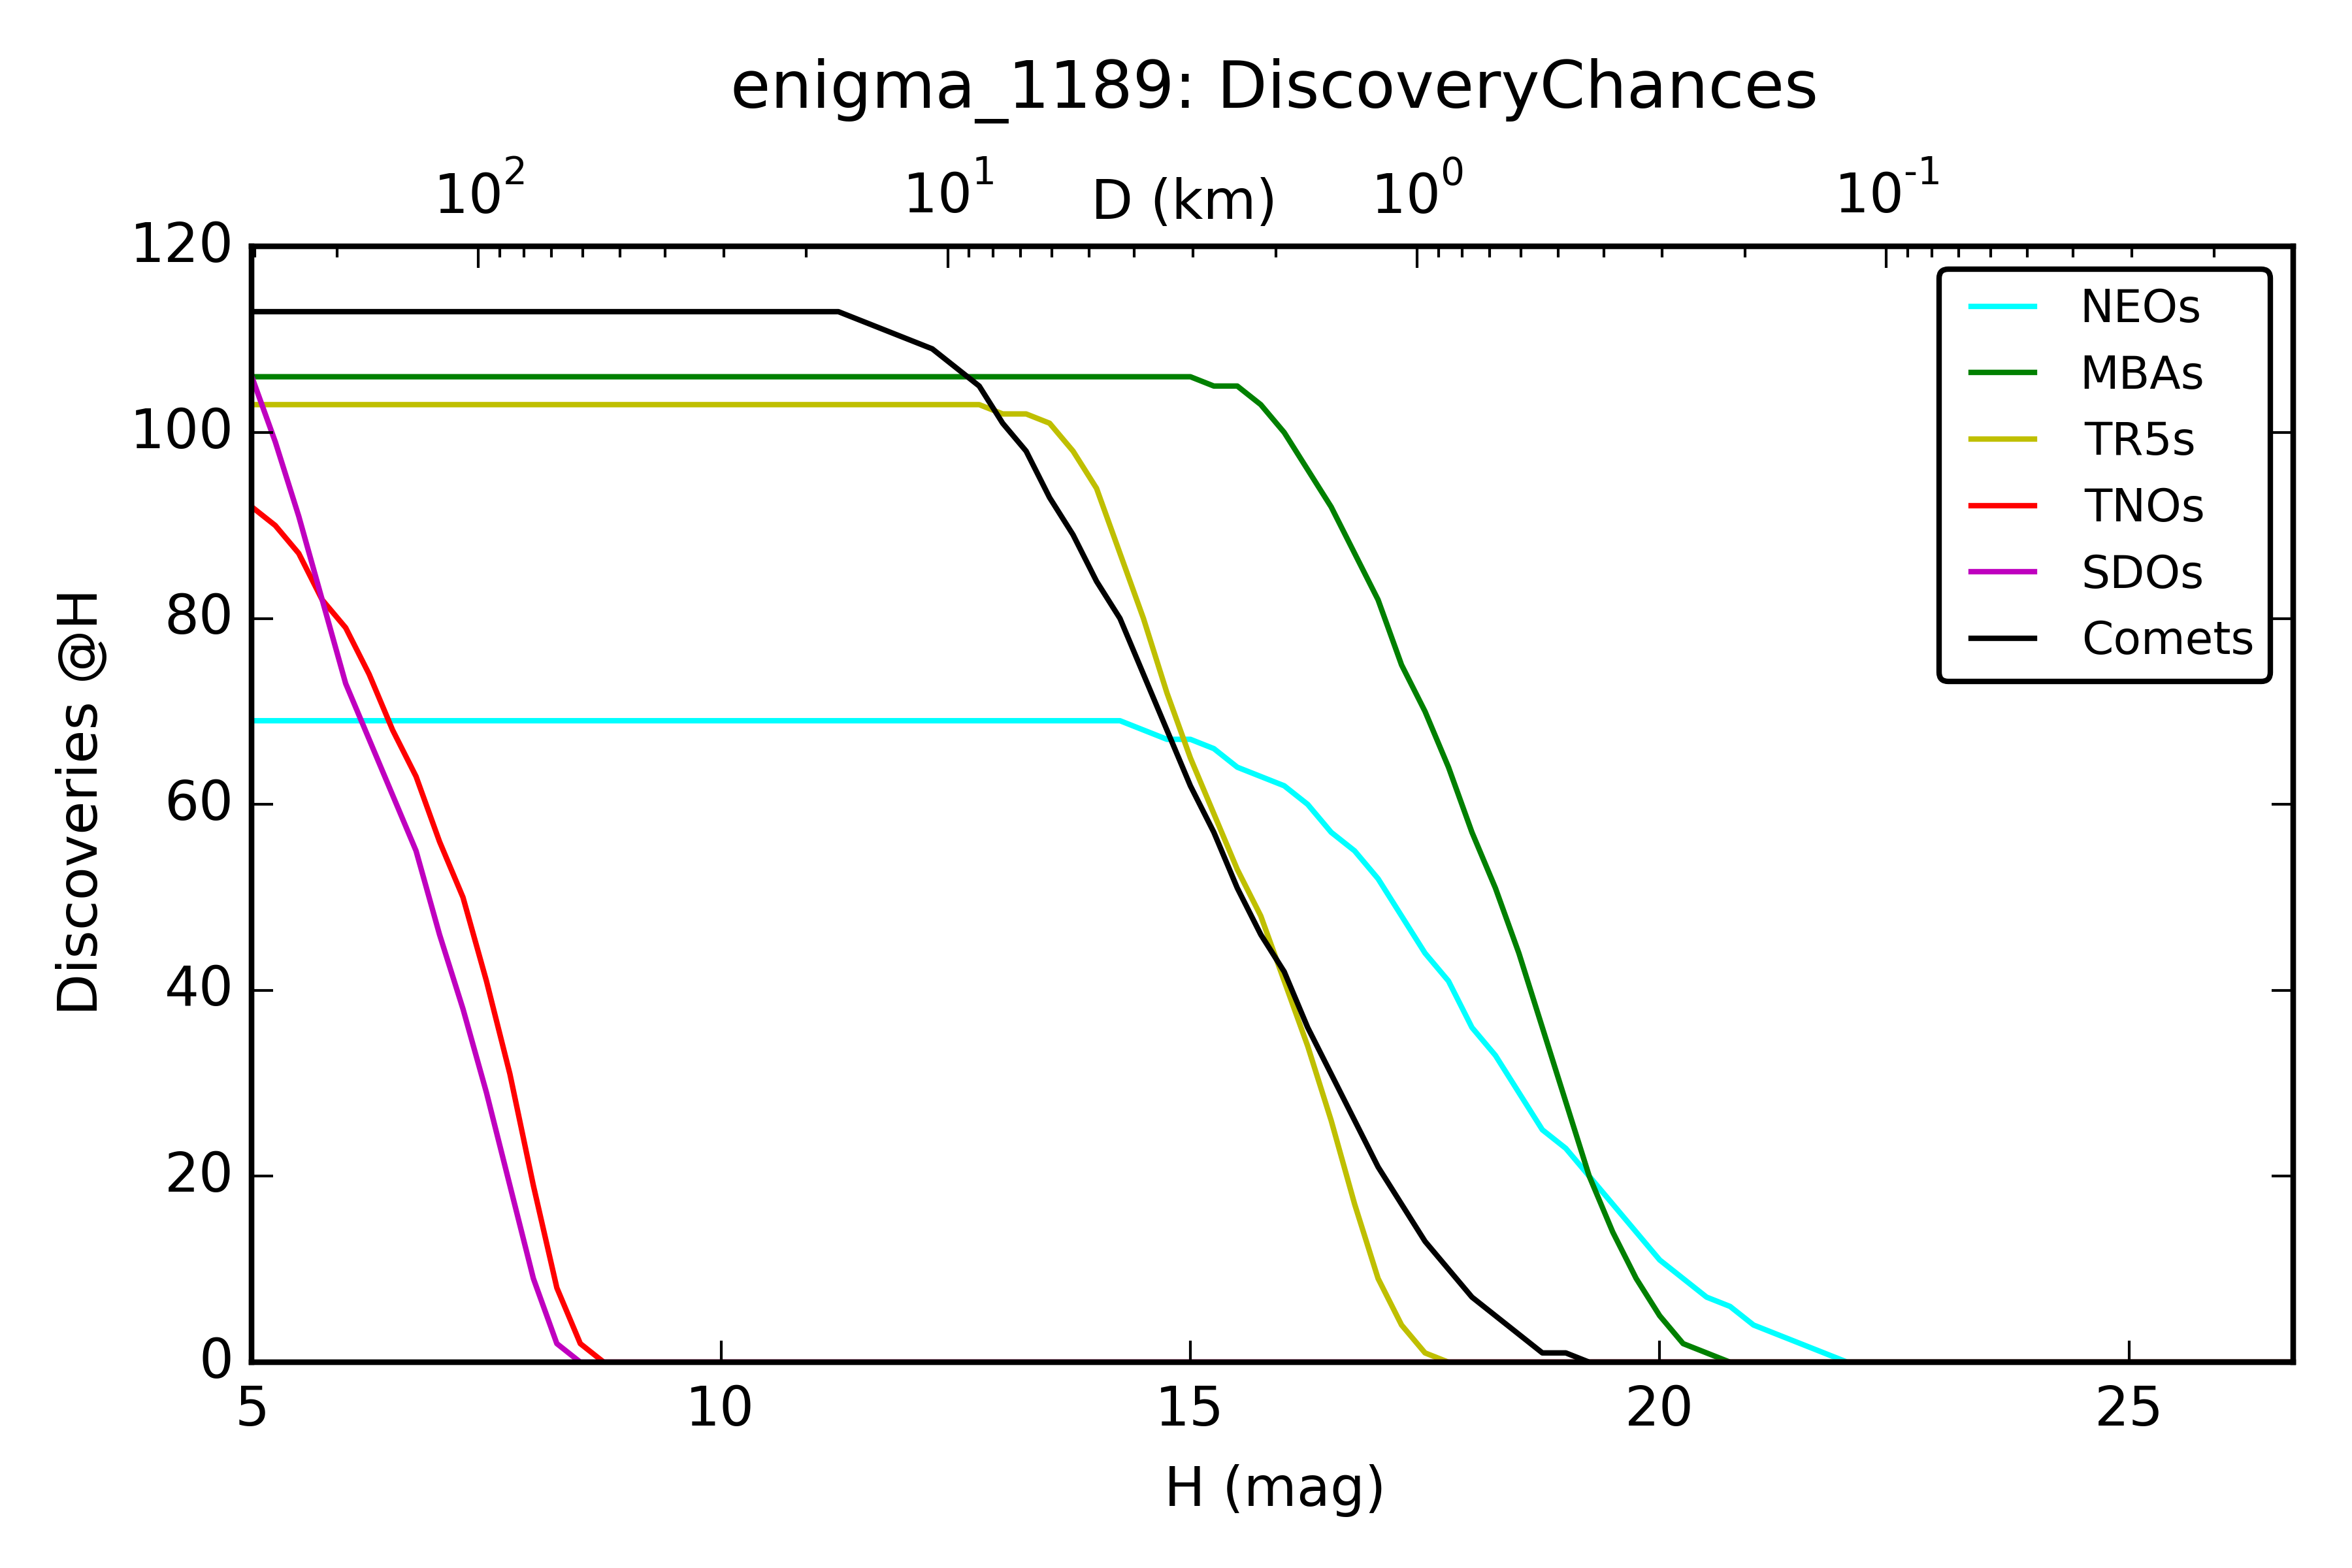
\includegraphics[width=3.5in]{figs/solarsystem/discoverychances}
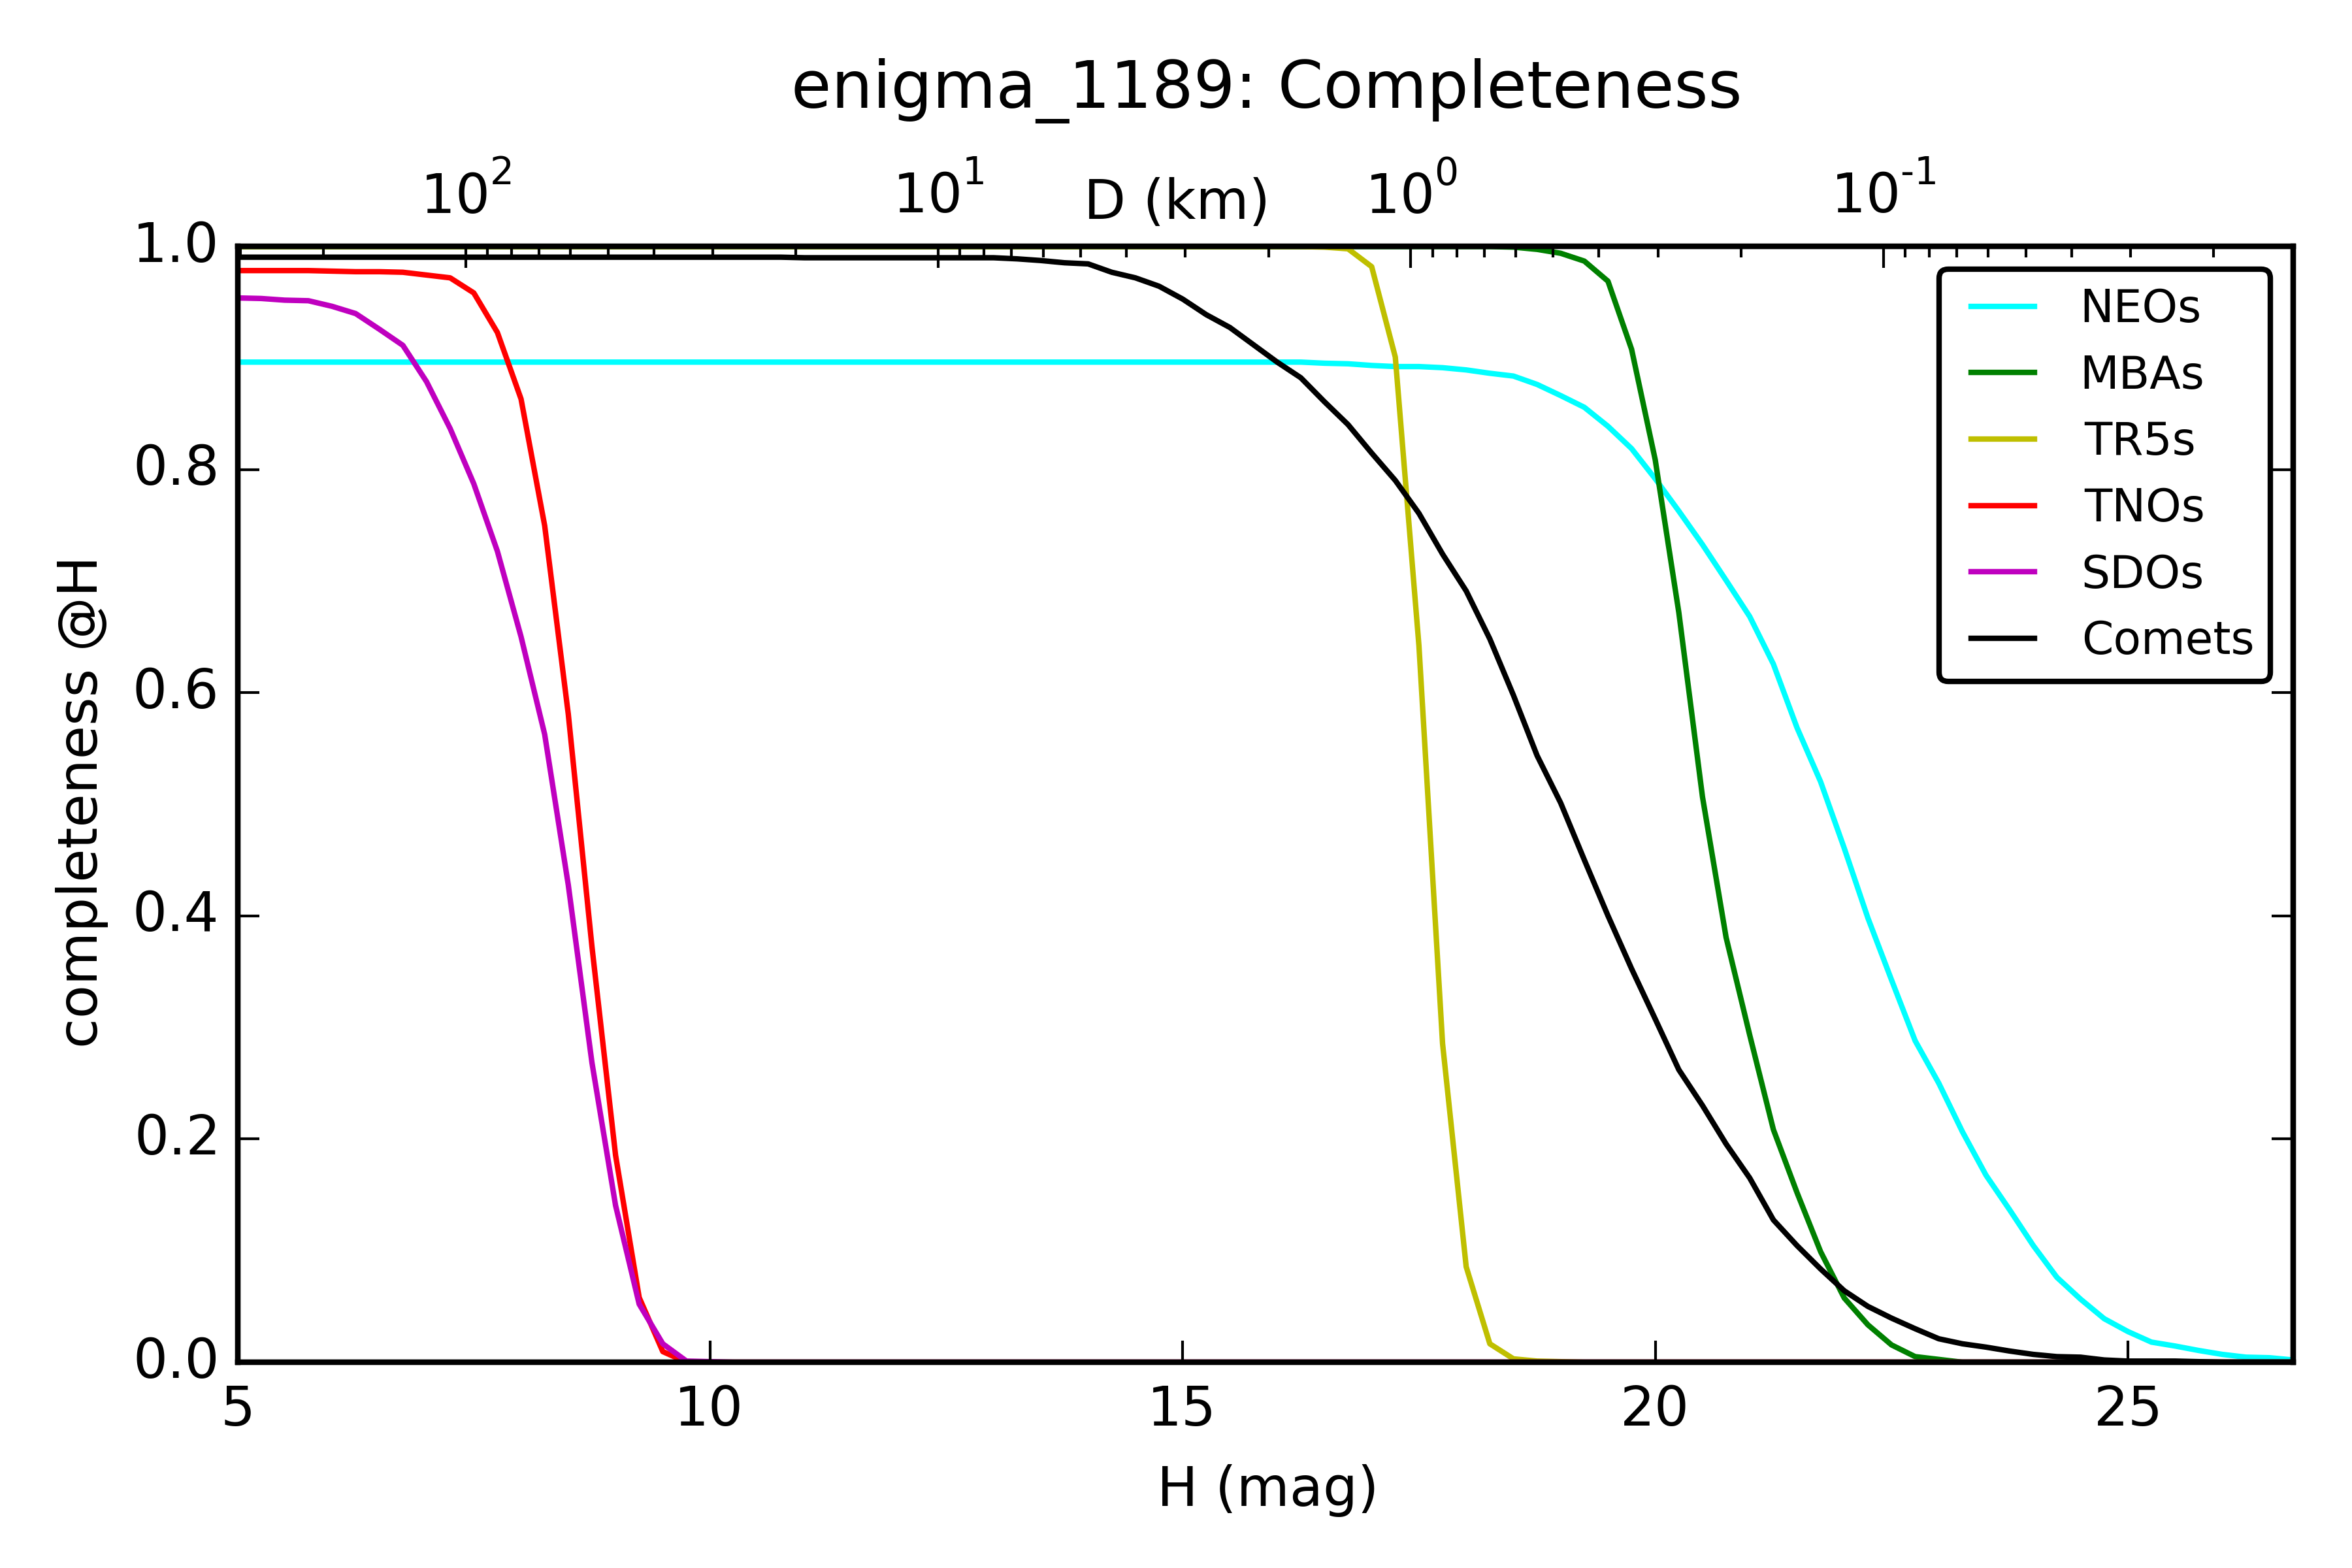
\includegraphics[width=3.5in]{figs/solarsystem/completeness}
\caption{Left: Number of discovery chances as a function of H
  (median value for all objects), assuming the minimum criteria for
  discovery - 2 visits per night within 90 minutes, repeated for 3
  nights within 15 days. Right: Resulting differential completeness across the
  entire population, assuming that only 1 discovery opportunity is
  required to `discover' each object. 
\label{standard_discovery}}
\end{figure}

Add table?


% --------------------------------------------------------------------

\subsection{Discussion}
\label{sec:\secname:discussion}

Add minimum completeness levels from solar system requirements
document



Discussion: what risks have been identified? What suggestions could be
made to improve this science project's figure of merit, and mitigate
the identified risks?



% ====================================================================

\section{Orbital Accuracy}
\def\secname{\chpname:orbits}\label{sec:\secname}


A short preamble goes here. What's the context for this science
project? Where does it fit in the big picture?

How secure is the orbit - is it going to hit us?
Libration amplitude distribution for TNOs?
Can we find it after X years for further study?
Can we identify the source region for NEOs within the main belt?

% --------------------------------------------------------------------

\subsection{Target measurements and discoveries}
\label{sec:\secname:targets}

Describe the discoveries and measurements you want to make.

Now, describe their response to the observing strategy. Qualitatively,
how will the science project be affected by the observing schedule and
conditions? In broad terms, how would we expect the observing strategy



% --------------------------------------------------------------------

\subsection{Metrics}
\label{sec:\secname:metrics}

Quantifying the response via MAF metrics: definition of the metrics,
and any derived overall figure of merit.


% --------------------------------------------------------------------

\subsection{OpSim Analysis}
\label{sec:\secname:analysis}

OpSim analysis: how good would the default observing strategy be, at
the time of writing for this science project?


% --------------------------------------------------------------------

\subsection{Discussion}
\label{sec:\secname:discussion}

Discussion: what risks have been identified? What suggestions could be
made to improve this science project's figure of merit, and mitigate
the identified risks?


% ====================================================================

\section{Detecting Activity}
\def\secname{\chpname:activity}\label{sec:\secname}


Comets are the remnant building blocks of the Solar System
that have been stored at cold temperatures beyond the ice
line, either in the Kuiper belt or the Oort cloud, since their
formation.  Measuring the evolution of cometary activity over
a range of heliocentric distances with LSST will allow to
understand the overall comet activity and to link these
observations with the physical and chemical conditions in the
early solar nebula during planet formation.  Comets are
classified in two main dynamical families, Jupiter Family
comets (JFCs) that have low-inclination orbits with periods
less than 20 years, and Long-period comets (LPCs) that
originate in the Oort Cloud at a distance of more than 10000
AU and have large orbital eccentricities and nearly isotropic
distribution of inclinations.  Currently there are over 400
Jupiter-family comets known, most of which are faint compared
with the LPCs.  LSST will observe about $10^4$ individual
comets repeatedly including measurements of known objects over
its 10-year survey \citep{2010PhDT.......241S}. The
determination of their activity levels at various heliocentric
distances will be used to study the time evolution of each
object individually and to find the connection between comet
families and their formation region in the Solar System.

Several cometary volatiles result in strong emission bands
excited by solar radiation that emit by resonant fluorescence
at optical and near-ultraviolet wavelengths.  The LSST $u$
filter peaks near the CN (0--0) emission band at 3880 \r{A}.
Although CN is not the most abundant daughter species from
cometary volatiles and the OH (0--0) emission band at 3080
\r{A} is generally stronger, CN production rates provide an
excellent proxy of the level of overall gas activity in
comets. Other bands such as $r$, $i$, and $z$ will detect
continuum brightness that is produced by reflected radiation
from dust particles in the coma. Thus, it will be possible to
obtain the evolution of the gas-to-dust production ratio at
high cadence as a function of heliocentric distance in
different comet families. The greatly increased sample size
compared with previous catalogs \citep{1995Icar..118..223A}
will allow for statistical comparison of the comet families
and to link them to other small body populations in the Solar
System.

% --------------------------------------------------------------------

\subsection{Target measurements and discoveries}
\label{sec:\secname:targets}

LSST will make an exceptionally large number of comet
observations.  About $10^4$ comets will be observed on average
of 50 times by LSST during its main survey, while a few objects
will be observed more than 1000 times
\citep{2010PhDT.......241S}.  Simulations of characteristic
comet orbits have shown that LSST will observe some Jupiter
Family comets (JFCs) hundreds of times over their full orbits
\citep{2010PhDT.......241S}.  Individual LPCs are predicted to
be observed by LSST with dozens of observations as they
approach or recede from the center of the Solar System or
during their perihelion passage.  Thus, these observations
will trace the onset of outgassing from quiescence at large
heliocentric distances and the decline of activity after
perihelion.  LSST will offer the unique opportunity to produce
a large database of CN production rates for the observed
comets that will vastly improve existing ones \citep[see
e.g.][]{1995Icar..118..223A,2012ApJ...758...29A}.

A recently discovered population of main-belt asteroids eject
dust and produce coma and tails giving them the appearance of
comets \citep{2012AJ....143...66J}.  This so-called main-belt
comets or active asteroids have the orbital characteristics of
asteroids with $T_J > 3$ and lose mass during part of their
orbits. The cometary activity observed in these objects may be
driven by primordial water water ice that is trapped near the
surface and sublimates when it is exposed to sunlight.
Main-belt comets are important because they may have been able to
preserve water ice despite the effect of solar radiation and
heating from the decay of short-lived radioactive nuclei.  The
asteroids in the outer regions of the main belt can therefore
have a substantial fraction of water and other volatiles that
may have supplied the volatile content of terrestrial planets.
Most of the main-belt-comets are faint with very weak comae
that are active during part of their orbits. Given the
expected flux sensitivity of LSST, the transient cometary
activity of main-belt asteroids will be observable including
many objects that could be below the detection limits of
current photometric surveys.  The LSST observations will thus
help to understand the overlap between different populations
in the Solar System such as the relationship between comets
and asteroids.

Now, describe their response to the observing strategy. Qualitatively,
how will the science project be affected by the observing schedule and
conditions? In broad terms, how would we expect the observing strategy
to be optimized for this science?


% --------------------------------------------------------------------

\subsection{Metrics}
\label{sec:\secname:metrics}

Quantifying the response via MAF metrics: definition of the metrics,
and any derived overall figure of merit.


% --------------------------------------------------------------------

\subsection{OpSim Analysis}
\label{sec:\secname:analysis}

OpSim analysis: how good would the default observing strategy be, at
the time of writing for this science project?


% --------------------------------------------------------------------

\subsection{Discussion}
\label{sec:\secname:discussion}

Discussion: what risks have been identified? What suggestions could be
made to improve this science project's figure of merit, and mitigate
the identified risks?

Different discussion / risks for each science case within this general metric?

% ====================================================================

\section{Measuring lightcurves/rotation periods}
\def\secname{\chpname:lightcurves}\label{sec:\secname}

Two Solar System science projects require
a series of photometric measurements. These
are (1) measuring lightcurves and therefore
shapes of minor bodies and (2) measuring
the colors and therefore compositions of
minor bodies. This section and the next describe
the science and the metrics for these
experiments.

% --------------------------------------------------------------------

\subsection{Target measurements and discoveries}
\label{sec:\secname:targets}

In general, minor bodies are aspherical,
and therefore observations of those bodies
produce lightcurves with non-zero amplitudes.
Constant monitoring of such a body would
reveal the detailed lightcurve, which can
be inverted to derive the effective observed
shape at that epoch.
Observations
over multiple epochs allow for observations
at different aspects, which can be used to
determine the three dimensional shape and pole
orientation of the minor body. All of this
information can be used to understand,
broadly, the orbital and physical evolution
of minor bodies in the Solar System.

LSST observations of minor bodies in the Solar System
will not, however, necessarily be dense in time
(with the exception of observations made in
Deep Drilling Fields; see below).
Therefore, lightcurves of minor bodies must
be combined across arbitrary rotational phase.
Without knowing the phase, the amplitude of
the lightcurve (a proxy for
asteroid shape) can simply be determined.
More complicated lightcurve inversion analysis
xxx ref xxx
can be carried out, given a sufficient number
of points.


% --------------------------------------------------------------------

\subsection{Metrics}
\label{sec:\secname:metrics}

The metric for lightcurve analysis
is therefore related to the number
of observations. The specific requirement
is
at least $\sim$100 measurements of an asteroid over
$\sim$years,
calibrated with a photometric accuracy of
$\sim$5\% (SNR=20)
or better. In these cases,
a coarse shape model can be derived.
The sparse data inversion gives correct results for both fast (0.2--2~h) and slow ($>$24~h) rotators (Durech et al.\ 2007, IAUS).



% --------------------------------------------------------------------

\subsection{OpSim Analysis}
\label{sec:\secname:analysis}

The present default OpSim does pretty well for this project.
Our estimate from existing metrics is that some $10^5$~main
belt asteroids will be observed $>$500~times in the 
nominal survey. 



% --------------------------------------------------------------------

\subsection{Discussion}
\label{sec:\secname:discussion}

The success of this experiment is predicated
on the idea that MOPS will work as advertised, 
that is, that the linking of tracklets and tracks
will be successful, so that each object's photometric
time series can be identified.

% ====================================================================

\section{Measuring colors}
\def\secname{\chpname:colors}\label{sec:\secname}

The varying compositions of asteroids result
in a range of optical colors. Sloan filters
in general are sufficiently diagnostic to
discriminate among different compositional
class xxx ref xxx. Therefore, when a Solar System
minor body is observed in griz (Solar System
objects are generally quite faint in u band
and many fewer will be detected; Y band xxx),
the color can be used to determine the composition
and, downstream, composition as a function of
asteroid size, family membership, orbital
elements, or many other parameters.

One obstacle to determining asteroid colors
is that asteroid rotation periods are
on the order of 2--20~hours, so that after
an initial measurement all further
measurements (in the same filter, or other
filters) are obtained at an arbitrary rotational
phase.
However, as described above, asteroid lightcurves
in a single band (presumably r band, which
will likely have the most detections) can be
derived. Any observing of that asteroid
in a different filter can be corrected
for the derived lightcurve brightness
offset at the time of the non-r band observation.
The intrinsic color of the asteroid can therefore
be measured.

% --------------------------------------------------------------------

\subsection{Target measurements and discoveries}
\label{sec:\secname:targets}



% --------------------------------------------------------------------

\subsection{Metrics}
\label{sec:\secname:metrics}

The metric of interest is the number
of observations in each band. If an asteroid has
more than $\sim$100 observations in r band,
then the lightcurve can be determined, and the
color can then be derived. The fidelity of the color
will depend on the number of measurements in
each band with SNR$>$20 (giving colors good to
5\%).



% --------------------------------------------------------------------

\subsection{OpSim Analysis}
\label{sec:\secname:analysis}

OpSim analysis: how good would the default observing strategy be, at
the time of writing for this science project?


% --------------------------------------------------------------------

\subsection{Discussion}
\label{sec:\secname:discussion}

Discussion: what risks have been identified? What suggestions could be
made to improve this science project's figure of merit, and mitigate
the identified risks?



% ====================================================================

\section{Deep Drilling Observations}
\def\secname{\chpname:dd}\label{sec:\secname}

Deep drilling observations provide the opportunity, via digital
shift-and-stack techniques, to discover Solar System Objects fainter
than the individual image limiting magnitude. These fainter objects
will be smaller, more distant, or lower albedo (or some combination of these)
than the general population found with individual images. Discovering smaller
objects is useful for constraining the size distribution to smaller
sizes; this provides constraints for collisional models and insights
into planetesimal formation. More distant objects are interesting in
terms of extending our understanding of each population over a wider
range of space; examples would be discovering very distant
Sedna-like objects or comets at larger distances from the Sun before
the onset of activity. Lower albedo objects may be useful to
understand the distribution of albedos, particularly to look for
trends with size.

Variations on the basic method of shift-and-stack have been used to
detect faint TNOs XXX Allen, Bernstein, Gladman, Fuentes, ?
XXX. Computational limitations on these methods mean that, roughly
and in general for images taken at opposition, images taken over the timespan of about an hour can be
combined and searched for main belt asteroids, and images taken over
the timespan of about 3 days can be combined and searched for more
distant objects like TNOs.

With extragalactic deep drilling fields as in the baseline enigma\_1189
run, where observations are taken in a series of filters (g, r, and i
would be useful for this purpose) each night, every three or four
days, we could use shift-and-stack to coadd the 50 images obtained in
gri bandpasses in a single night. This would allow detection of
objects about 2 magnitudes fainter than in the regular survey, or
approximately $r=26.5$.  This is cool and a range of ecliptic
latitudes is interesting.  But, we would like to do better.

Recap solar system DD white paper.

Describe how we will evaluate DD proposal, with TNO population +
estimate on number of times objects observed (but not doing actual
shift-and-stack). Need large-i populations to test if useful, probably.


\navigationbar

% ====================================================================
